\documentclass{article}
\usepackage{graphicx}
\usepackage{amsmath}
\usepackage{cite}
\usepackage{color}
\usepackage{enumitem}
\usepackage{hyperref}
\usepackage{natbib}
\usepackage{tabularx}
\usepackage{natbib}
\usepackage{ragged2e}

\title{\textbf{La dis-informazione}}
\author{\texttt{Alessandro Meloni GEPID}}
\date{10/12/2023}

\begin{document}
\maketitle
    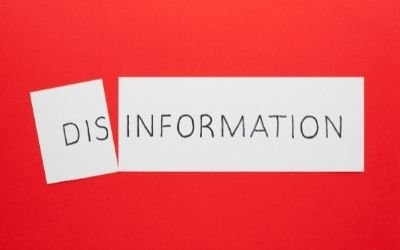
\includegraphics[width = 0.6\linewidth]{Immagini/disinformation.jpeg}
\centering \tableofcontents
\newpage \section{Introduzione}
\flushleft
\begin{justify}
    Questo articolo avrà prevalentemente la finalità di provare a mettere in chiaro cosa si intenda per disinformazione; e le varie sfaccettature che questo concetto può assumere.
    Faremo in modo di dare chiarezza in quanto la disinformazione ha di per sè una finalità negativa e di sviamento da ciò che è corretto, ma anche la sua forma non sempre risulta essere compresa agli occhi dei lettori.
    Innanzitutto faremo una piccola descrizione del concetto di disinformazione e le sue varie sfaccettature; successivamente analizzeremo una survey effettuata da parte dell'Unesco nel 2023, e, pubblicata dal \href{https://www.theguardian.com/technology/2023/nov/07/85-of-people-worry-about-online-disinformation-global-survey-finds}{The Guardian}\label{:articolo} come articolo nella loro pagina internet. Questo sarà seguito da un piccolo sondaggio fatto su un campione di X persone, provando a comprendere, almeno in Italia, quale possa essere la tendenza di percezione di questo concetto da parte della popolazione.
    Faremo e spiegheremo dei grafici risultanti dalla survey, così da comprendere quanto possano variare le percezioni sulla disinformazione sulla base di caratteristiche personali. 
    Seguirà successivamente una comparazione con alcuni dati relativi alla presenza oggettiva di fake news, così da capire se le percezioni delle persone, poi, coincidono con la frequenza oggettiva del fenomeno all'interno dei vari media.
    In conclusione, vedremo i risultati che ha dato questa ricerca, così da dare dei consigli su come riconoscere informazioni da dis-informazioni, con lo scopo di creare una maggiore consapevolezza e sicurezza nell'utente/lettore medio, evitando che questo fenomeno possa davvero portare al fine per cui la notizia viene diffusa.
    
\end{justify}
\begin{center}
\newpage \section{Il fenomeno della disinformazione}
\end{center}
\begin{justify}
    La disinformazione è quel fenomeno che viene studiato prevalentemente negli ambiti di scienze della comunicazione, ma che può espandersi a tanti rami.
    L'etimologia del termine risale al 1980, appunto perché venne per la prima volta utilizzato il termine russo \textit{dezinformatzija}, che si riferisce a "un'arma" che venne istituita dal KGB, e che consisteva semplicemente nel creare un ufficio ad hoc finalizzato alla diffusione e gestione della disinformazione, come attività di intelligence.\citep{DisWiki}\\
    Quindi dalla creazione dell'ufficio, iniziò a diffondersi questa terminologia, andando a colpire tutti gli stati mondiali, chi può e chi meno.
\end{justify}

\centering\subsection{Cos'è la disinformazione?}
\begin{justify}
    La disinformazione è un concetto molto ampio, e bisogna subito mettere in chiaro il fatto che non si riferisca esclusivamente a intenzioni malevoli, di fatto, è giusto, come definito dalla sociologa \texttt{Claire Wardle}, suddividere questo concetto in tre ramificazioni, comprendendo: Ragioni economiche dietro fake news? (Twitter che perde il 15\%  Trigger come elemento scatenante.
    Dragonfly search engine
\begin{itemize}
    \item Disinformazione: la diffusione di notizie false con lo scopo specifico di trarre in inganno e sviare singoli soggetti, organizzazioni di persone o popolazioni intere: molte volte con finalità strettamente collegate ad ambito politico, finanziario ed interessi egoistici.
    \item Misinformazione: questo termine viene preso dall'inglese "misinformation" e indica un'informazione che di per sè è falsa, ma senza l'effettiva finalità di nuocere altrui soggetti da parte di colui o coloro che la diffondono. Certe volte è collegata alla diffusione di pezzi di informazione di un contenuto più ampio, senza sapere che esiste questo contenuto;
    \item Malinformazione: questo termine si distacca dalla normale definizione di "notizia falsa", però è opportuno ricomprenderla perchè ha come contenuto una notizia vera, ma che viene diffusa senza specificare il contesto, così da arrecare danno ad uno specifico soggetto o soggetti coinvolti nella notizia. \citep{wardle2018information}
\end{itemize}
In generale è conveniente, per le tech companies, la diffusione di questi fenomeni, perché, oltre a creare una maggiore diffusione del contenuto porta anche più persone a discuterne, indipendente dal fatto che sia un contenuto positivo o negativo.
\end{justify}


\centering\newpage\subsection{Analisi dati:}
\begin{justify}    
Come già accennato nell'introduzione andremo ad analizzare precisamente una sezione della survey che è stata fatta da parte dell'UNESCO in collaborazione con IPSOS, i cui dati sono stati raccolti dal 22 Agosto al 25 Settembre 2023, e, pubblicato dal The Guardian in data 7 Novembre 2023\ref{:articolo}. \citep{Unesco}
Il campione analizzato è stato formato da 500 soggetti per ogni Stato dei 16 coinvolti, per una totalità campionaria di 8000 soggetti (con un totale di popolazione pari a \textit{2.579.400.000}).
Questi 16 Stati sono stati suddivisi sulla base del loro HDI (indice di sviluppo umano), e, ogni Stato, è stato scelto in previsione delle elezioni del 2024 (infatti vediamo che non c'è l'Italia).
Come definito dall'UNESCO, la finalità è stata quella di visualizzare e analizzare, dando voce ai cittadini, quanto venga percepito l'impatto della disinformazione e degli hate speech durante la loro vita quotidiana. D'altro canto, molto importante, è stata la decisione di fare questa survey prima delle elezioni, proprio per comprendere se in questi casi potrebbe essere sentita una maggiore diffusione di questi due fenomeni.
\end{justify}

\centering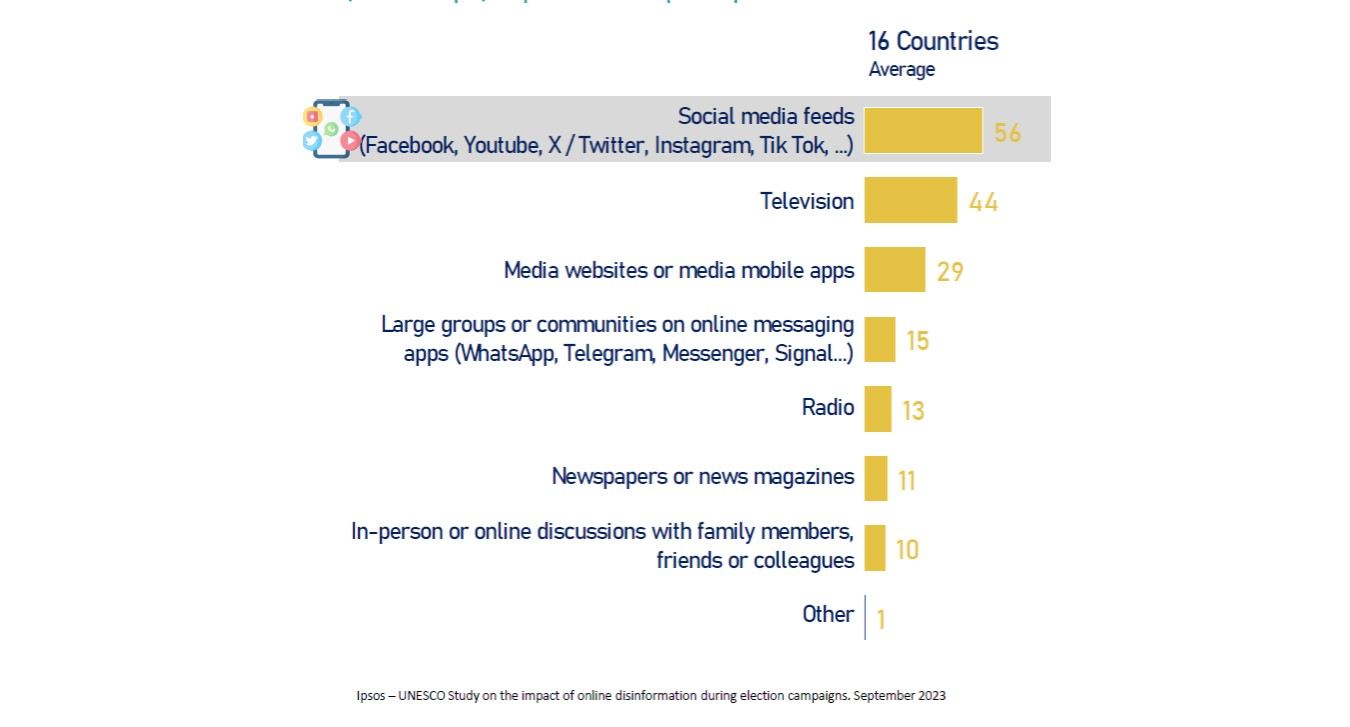
\includegraphics[width=0.5\linewidth]{Immagini/Grafico1.jpg}\\
    \begin{justify}
    Questo è il primo grafico che andremo ad analizzare dalla quale è stata posta la seguente domanda: "Qual è lo strumento che utilizzi di più per reperire news e informazioni?".
    Innanzitutto vediamo che gli strumenti che prevalgono sono i social network, con un distacco abbastanza sostanzioso dalla TV o altre Media inseriti all'interno dello stesso. Sicuramente questo ci sottolinea come, con l'avvento della digitalizzazione e dei social, le persone tendano più a informarsi con queste tecnologiche, perchè è molto più facile e veloce reperire le informazioni, visto che possono essere consultate in qualsiasi momento, al contrario della TV, perchè dovresti andare al canale specifico e aspettare che facciano rivedere il servizio (se sei fortunato).
\begin{center}
    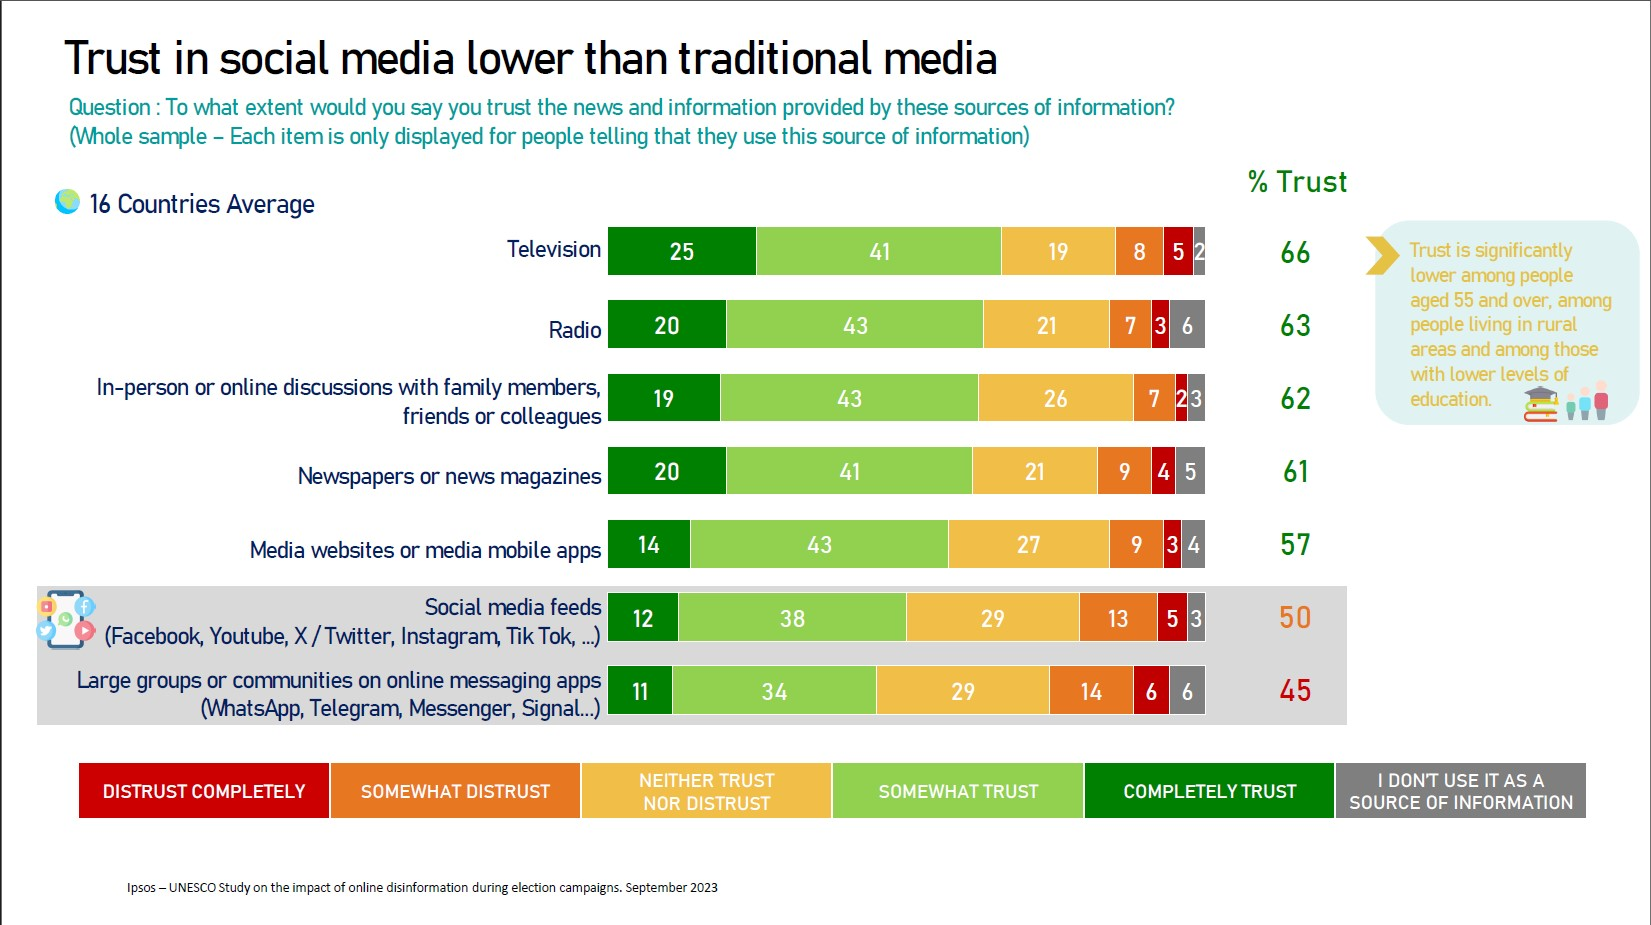
\includegraphics[width=0.5\linewidth]{Immagini/Grafico2.jpg}\\
\end{center}
    Oltre al fatto di capire come le persone si informano, bisogna comprendere anche il grado di fiducia che gli utenti danno a queste informazioni; invero, il secondo grafico rappresenta il grado di fiducia che le persone hanno rispetto agli stessi media che sono stati proposti nella prima domanda.
    Attraverso una scala di risposta inserita in riferimento a questa domanda, è stato dato maggiore spazio di risposta agli intervistati (metodo che vedremo verrà confermato anche nei prossimi grafici).
    Già da qua vediamo un controsenso, perchè gli intervistati si fidano di più dei media Televisivi, Radio, Discussioni offline, Giornali fisici e online; rispetto ai social media; mentre prima i social erano considerati come il mezzo prevalente nel reperire informazioni. A rigor di logica, quello che utilizzi di più dovrebbe coincidere anche con quello di cui ti fidi di più, invece in questo caso non accade. Potremo intuire che i social vengano utilizzati più in maniera ricreativa e ludica, ed è per questo che si presenta questa contraddizione.
    \end{justify}

\centering\subsection{L'impatto della disinformazione nella vita delle persone}
\begin{justify}
    
\end{justify}
\centering
\newpage\section{Riflessioni e conclusioni}

\newpage\bibliography{Bibliografia}
\bibliographystyle{unsrtnat}
\end{document}